\section{Date: 2026-10-17}
\noindent \textbf{Series ID: QTAXT01QTAXCAT3INNO} 

\noindent This series is titled State Tax Collections: T01 Property Taxes for Indiana and has a frequency of Quarterly. The units are Millions of U.S. Dollars and the seasonal adjustment is Not Seasonally Adjusted.The observation start date is 1994-01-01 and the observation end date is 2026-04-01.The popularity of this series is 1. \\ 

\noindent \textbf{Series ID: NPTLTL19} 

\noindent This series is titled Nonperforming Total Loans (past due 90+ days plus nonaccrual) to Total Loans, Banks with Total Assets up to \$300M, Pacific Census Division (DISCONTINUED) and has a frequency of Quarterly, End of Period. The units are Percent and the seasonal adjustment is Not Seasonally Adjusted.The observation start date is 1988-01-01 and the observation end date is 2020-07-01.The popularity of this series is 1. \\ 

\subsection{Raw Regression}
\noindent Regresses the two series against each other directly. A significant result here can come just as easily from both series sharing a long-run trend as from any real relationship.

\begin{center}
\begin{tabular}{lclc}
\toprule
\textbf{Dep. Variable:}                   & value\_fred\_NPTLTL19 & \textbf{  R-squared:         } &     0.272   \\
\textbf{Model:}                           &          OLS          & \textbf{  Adj. R-squared:    } &     0.266   \\
\textbf{Method:}                          &     Least Squares     & \textbf{  F-statistic:       } &     39.32   \\
\textbf{Date:}                            &    Sat, 17 Oct 2026   & \textbf{  Prob (F-statistic):} &  8.12e-09   \\
\textbf{Time:}                            &        14:31:31       & \textbf{  Log-Likelihood:    } &   -164.09   \\
\textbf{No. Observations:}                &            107        & \textbf{  AIC:               } &     332.2   \\
\textbf{Df Residuals:}                    &            105        & \textbf{  BIC:               } &     337.5   \\
\textbf{Df Model:}                        &              1        & \textbf{                     } &             \\
\textbf{Covariance Type:}                 &       nonrobust       & \textbf{                     } &             \\
\bottomrule
\end{tabular}
\begin{tabular}{lcccccc}
                                          & \textbf{coef} & \textbf{std err} & \textbf{t} & \textbf{P$> |$t$|$} & \textbf{[0.025} & \textbf{0.975]}  \\
\midrule
\textbf{const}                            &       2.6515  &        0.204     &    12.989  &         0.000        &        2.247    &        3.056     \\
\textbf{value\_fred\_QTAXT01QTAXCAT3INNO} &      -0.6722  &        0.107     &    -6.271  &         0.000        &       -0.885    &       -0.460     \\
\bottomrule
\end{tabular}
\begin{tabular}{lclc}
\textbf{Omnibus:}       &  5.363 & \textbf{  Durbin-Watson:     } &    0.313  \\
\textbf{Prob(Omnibus):} &  0.068 & \textbf{  Jarque-Bera (JB):  } &    5.479  \\
\textbf{Skew:}          &  0.537 & \textbf{  Prob(JB):          } &   0.0646  \\
\textbf{Kurtosis:}      &  2.723 & \textbf{  Cond. No.          } &     4.30  \\
\bottomrule
\end{tabular}
%\caption{OLS Regression Results}
\end{center}

Notes: \newline
 [1] Standard Errors assume that the covariance matrix of the errors is correctly specified.

\begin{figure}
\centering
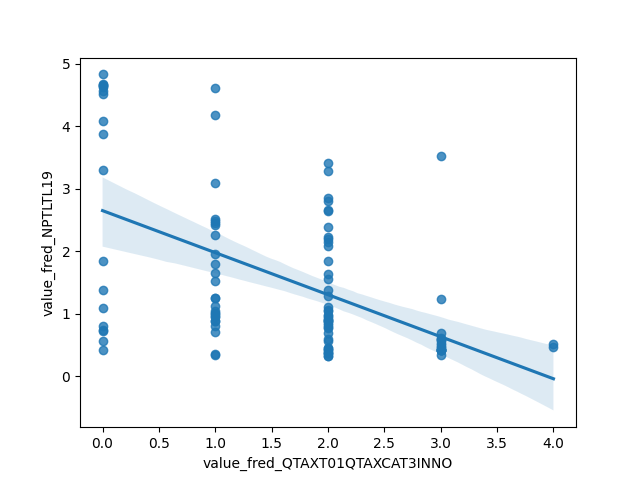
\includegraphics[scale = 0.9]{plots/plot_2026-10-17.png}
\caption{Raw Regression Plot for 2026-10-17}
\end{figure}
\newpage
\subsection{Detrended Regression}
\noindent Regresses the residuals of each series after removing its own linear time trend, so a shared trend can no longer drive the result on its own. A relationship that stays significant here is better evidence of a genuine link between the two series.

\begin{center}
\begin{tabular}{lclc}
\toprule
\textbf{Dep. Variable:}                              & value\_fred\_NPTLTL19\_detrended & \textbf{  R-squared:         } &     0.283   \\
\textbf{Model:}                                      &               OLS                & \textbf{  Adj. R-squared:    } &     0.276   \\
\textbf{Method:}                                     &          Least Squares           & \textbf{  F-statistic:       } &     41.41   \\
\textbf{Date:}                                       &         Sat, 17 Oct 2026         & \textbf{  Prob (F-statistic):} &  3.75e-09   \\
\textbf{Time:}                                       &             14:31:31             & \textbf{  Log-Likelihood:    } &   -163.18   \\
\textbf{No. Observations:}                           &                 107              & \textbf{  AIC:               } &     330.4   \\
\textbf{Df Residuals:}                               &                 105              & \textbf{  BIC:               } &     335.7   \\
\textbf{Df Model:}                                   &                   1              & \textbf{                     } &             \\
\textbf{Covariance Type:}                            &            nonrobust             & \textbf{                     } &             \\
\bottomrule
\end{tabular}
\begin{tabular}{lcccccc}
                                                     & \textbf{coef} & \textbf{std err} & \textbf{t} & \textbf{P$> |$t$|$} & \textbf{[0.025} & \textbf{0.975]}  \\
\midrule
\textbf{const}                                       &   -5.444e-14  &        0.109     & -5.02e-13  &         1.000        &       -0.215    &        0.215     \\
\textbf{value\_fred\_QTAXT01QTAXCAT3INNO\_detrended} &      -0.7171  &        0.111     &    -6.435  &         0.000        &       -0.938    &       -0.496     \\
\bottomrule
\end{tabular}
\begin{tabular}{lclc}
\textbf{Omnibus:}       &  3.007 & \textbf{  Durbin-Watson:     } &    0.359  \\
\textbf{Prob(Omnibus):} &  0.222 & \textbf{  Jarque-Bera (JB):  } &    2.982  \\
\textbf{Skew:}          &  0.397 & \textbf{  Prob(JB):          } &    0.225  \\
\textbf{Kurtosis:}      &  2.804 & \textbf{  Cond. No.          } &     1.03  \\
\bottomrule
\end{tabular}
%\caption{OLS Regression Results}
\end{center}

Notes: \newline
 [1] Standard Errors assume that the covariance matrix of the errors is correctly specified.

\begin{figure}
\centering
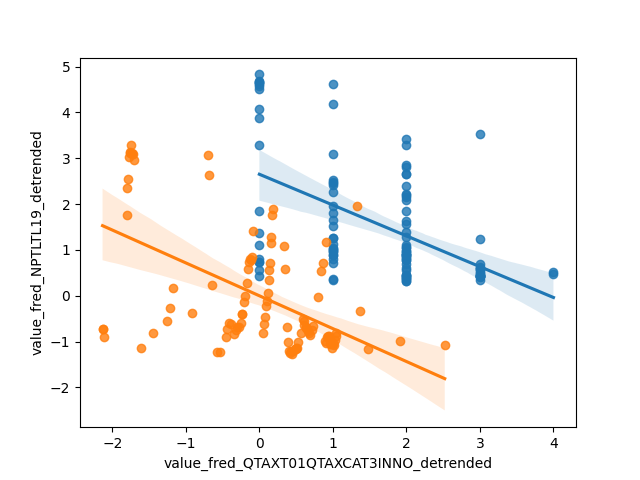
\includegraphics[scale = 0.9]{plots/plot_2026-10-17_detrended.png}
\caption{Detrended Regression Plot for 2026-10-17}
\end{figure}
\newpage
